\documentclass[multi=page, border=1cm]{standalone}

\usepackage{graphicx}
\usepackage{amsmath}

\newcommand{\card}[2]{
    \begin{page}\scalebox{4}{#1}\end{page}
    \begin{page}\scalebox{4}{#2}\end{page}
}
\newcommand{\mathcard}[2]{\card{#1}{\(\displaystyle #2\)}}

\pagestyle{empty}

\begin{document}

\mathcard{Entropy}{H = \sum_i{p_i\log_2{\frac{1}{p_i}}}}
\mathcard{Conditional Entropy}{H(X \mid Y) = \sum_{x,y}{ p(x, y) \log\frac{1}{p(x \mid y)} }}
\mathcard{Mutual Information}{I(X;Y) = \sum_{x,y}{ p(x,y)\log\frac{p(x,y)}{p(x)p(y)} }}

\mathcard{Independence Bound on Entropy}{H(X_1,...,X_n) \leq \sum_i{ H(X_i) }}
\mathcard{Fano's Inequality}{P_e \geq \frac{1 - H(X \mid Y)}{\log{|X|}}}
\card{Data Processing Inequality}
{
    If \(X \rightarrow Y \rightarrow Z\) for some transformation \(\rightarrow\), then \(I(X;Y) \geq I(X;Z)\).
}

\mathcard{Mutual Information Distance}{D(X,Y) = H(X,Y) - I(X;Y)}
\mathcard{Kullback-Leibler Distance}{D_{KL}(p \mid\mid q) = \sum_x{ p(x) \log\frac{p(x)}{q(x)} }}

\card{Markov Process Entropy}{Average of the entropy of each state weighted by occupancy probability.}

\card{Code Rate}{\(R\), weighted average cost of sending a symbol in bits/symbol.}
\card{Average Codeword Length}{Same as Code Rate: bits per symbol.}

\card{Efficiency of a code}{Information content of each bit: \(\displaystyle \eta = \frac{H}{R}\)}
\card{Prefix Property}{No codeword is the prefix of a longer codeword: equivalent to unique decodability}
\card{Relationship between uniquely decodable and instantaneous}{Instantaneous implies Uniquely Decodable}

\card{Shannon's Source-Coding Theorem}
{
    \begin{tabular}{c}
    For a source with entropy \(H\) and \(\varepsilon>0\), there's a uniquely \\
    decodable code such that \(R = H + \varepsilon\) as \(\varepsilon \rightarrow 0\)
    \end{tabular}
}

\card{Huffman Code}{Optimal prefix code: binary tree, combine nodes and sum probabilities.}

\card{Kraft McMillan Inequality}{\(\displaystyle \sum_{i=1}^N{\frac{1}{2^{c_i}}} \leq 1\) is necessary but not sufficient for instantaneous.}

\card{Channel Matrix}{\(p(y_j \mid x_i)\), probability of getting output \(y_j\) given input \(x_i\).}
\mathcard{Probability of getting a symbol \(y\) from a channel}{\sum_x{ p(y \mid x)p(x) }}

\card{Channel Capacity}{Maximum mutual information over all possible input distributions}

\card{Shannon's Channel-Coding Theorem}
{
    \begin{tabular}{c}
    For a channel with capacity \(C\) and symbol source with entropy \(H \leq C\),\\
    there's a coding scheme such that the source is reliably transmitted \\
    with arbitrarily small error.
    \end{tabular}
}

\card{7/4 Hamming Code}{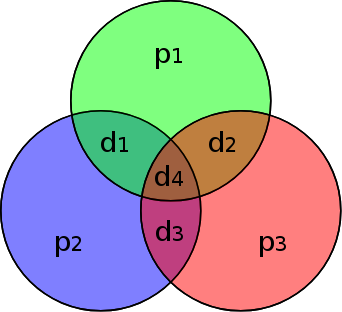
\includegraphics[width=4cm]{hamming74.png}}
\card{Perfect Error Correcting Code}{Code using \(m\) bits to correct \(2^m - 1\) \textbf{error patterns}.}

\card{Fourier Series}
{
    \renewcommand{\arraystretch}{3}
    \begin{tabular}{c}
    \setlength{}
    \(\displaystyle \frac{a_0}{2} + \sum_{n=1}^\infty\Big[ a_n\cos(nx) + b_n\sin(nx) \Big]\) \\
    \(\displaystyle \Bigg\{ \frac{1}{\sqrt{2}},\;\sin(x),\;\cos(x),\;\sin(2x),\;\cos(2x),\;... \Bigg\}\) \\
    \(\displaystyle a_n = \frac{1}{\pi} \int_{-\pi}^\pi{f(x)\cos(nx)\,dx}, \qquad n=0,1,2,...\) \\
    \(\displaystyle b_n = \frac{1}{\pi} \int_{-\pi}^\pi{f(x)\sin(nx)\,dx}, \qquad n=1,2,3,...\)
    \end{tabular}
}

\card{Lowpass, bandpass, highpass}{Filter low, range, high frequencies}

\card{Distribution maximising channel entropy for fixed variance \(\sigma^2\)?}{Gaussian: also maximises mutual information, so defines the channel capacity.}

\mathcard{Maximum entropy of a Gaussian}{H = \frac{1}{2}\log(2\pi e \sigma^2)}

\mathcard{Capacity of an AWGN channel with spectral power density \(N_0\)}{C = \int_{-\infty}^\infty{ \log(1 + \frac{P}{WN_0})\,d\omega }}
\mathcard{Capacity of a gaussian-noise channel}{C = \int_{-\infty}^\infty{ \log(1 + SNR(\omega))\,d\omega }}

\mathcard{Power Spectral Density}{N_0}
\mathcard{Signal-to-Noise Ratio}{\frac{P}{WN_0}}

\mathcard{Fourier Transform}{F(\omega) = \frac{1}{2\pi} \int_{-\infty}^\infty{ f(t) e^{-i\omega t} dt }}
\mathcard{Inverse Fourier Transform}{f(t) = \int_{-\infty}^\infty{ F(\omega) e^{i\omega t} d\omega }}

\card{Self-Fourier}{Fourier transformation doesn't affect the form of the function.}

\mathcard{Convolution}{(f * g)(x) = \int_{-\infty}^\infty{ f(x - y)g(y)\,dy }}

\card{Signal Modulation}{Fourier transform of \(f(t)e^{ict}\) is \(F(\omega - c)\).}

\card{Nyquist's Sampling Theorem}{Can completely reconstruct a function if we sample it at least 2\(W\).}
\card{Logan's Theorem}{For a signal with \(2W_L \geq W_H\), can reconstuct the function from just the zero-crossings.}

\card{Gabor's Information Diagram}{Frequency vs Time, signal area is \(\displaystyle >\frac{1}{4\pi}\).}
\card{Gabor Wavelet}{Helical functions scaled by a Gaussian. Have optimal minimal area, but non-orthogonal.}

\card{RLE}{Remove redundancy in strings of repeating values.}
\card{Predictive Coding}{Record deviations from a prediction rather than actual sample values.}
\card{Dictionary Compression}{Sparsity of language means number of useful strings is way fewer than address space.}
\card{LZW Algorithm}{Dictionary compression algo, two passes.}

\card{Dyadic Wavelet}{Mother wavelet \(\Psi(x)\) which spawns daughters \(\Psi_{jk}(x)\) which are transforms of the mother.}

\card{Kolmogorov Complexity}{The length of the shortest program that can reproduce the string.}
\card{K-incompressible}{Kolmogorov Complexity tends to the length of the string in the limit to \(\infty\).}

\end{document}